\subsection{Кеплеровы элементы орбиты}

\begin{wrapfigure}[11]{r}{0.45\tw}
    \centering
    \vspace{-0.7pc}
    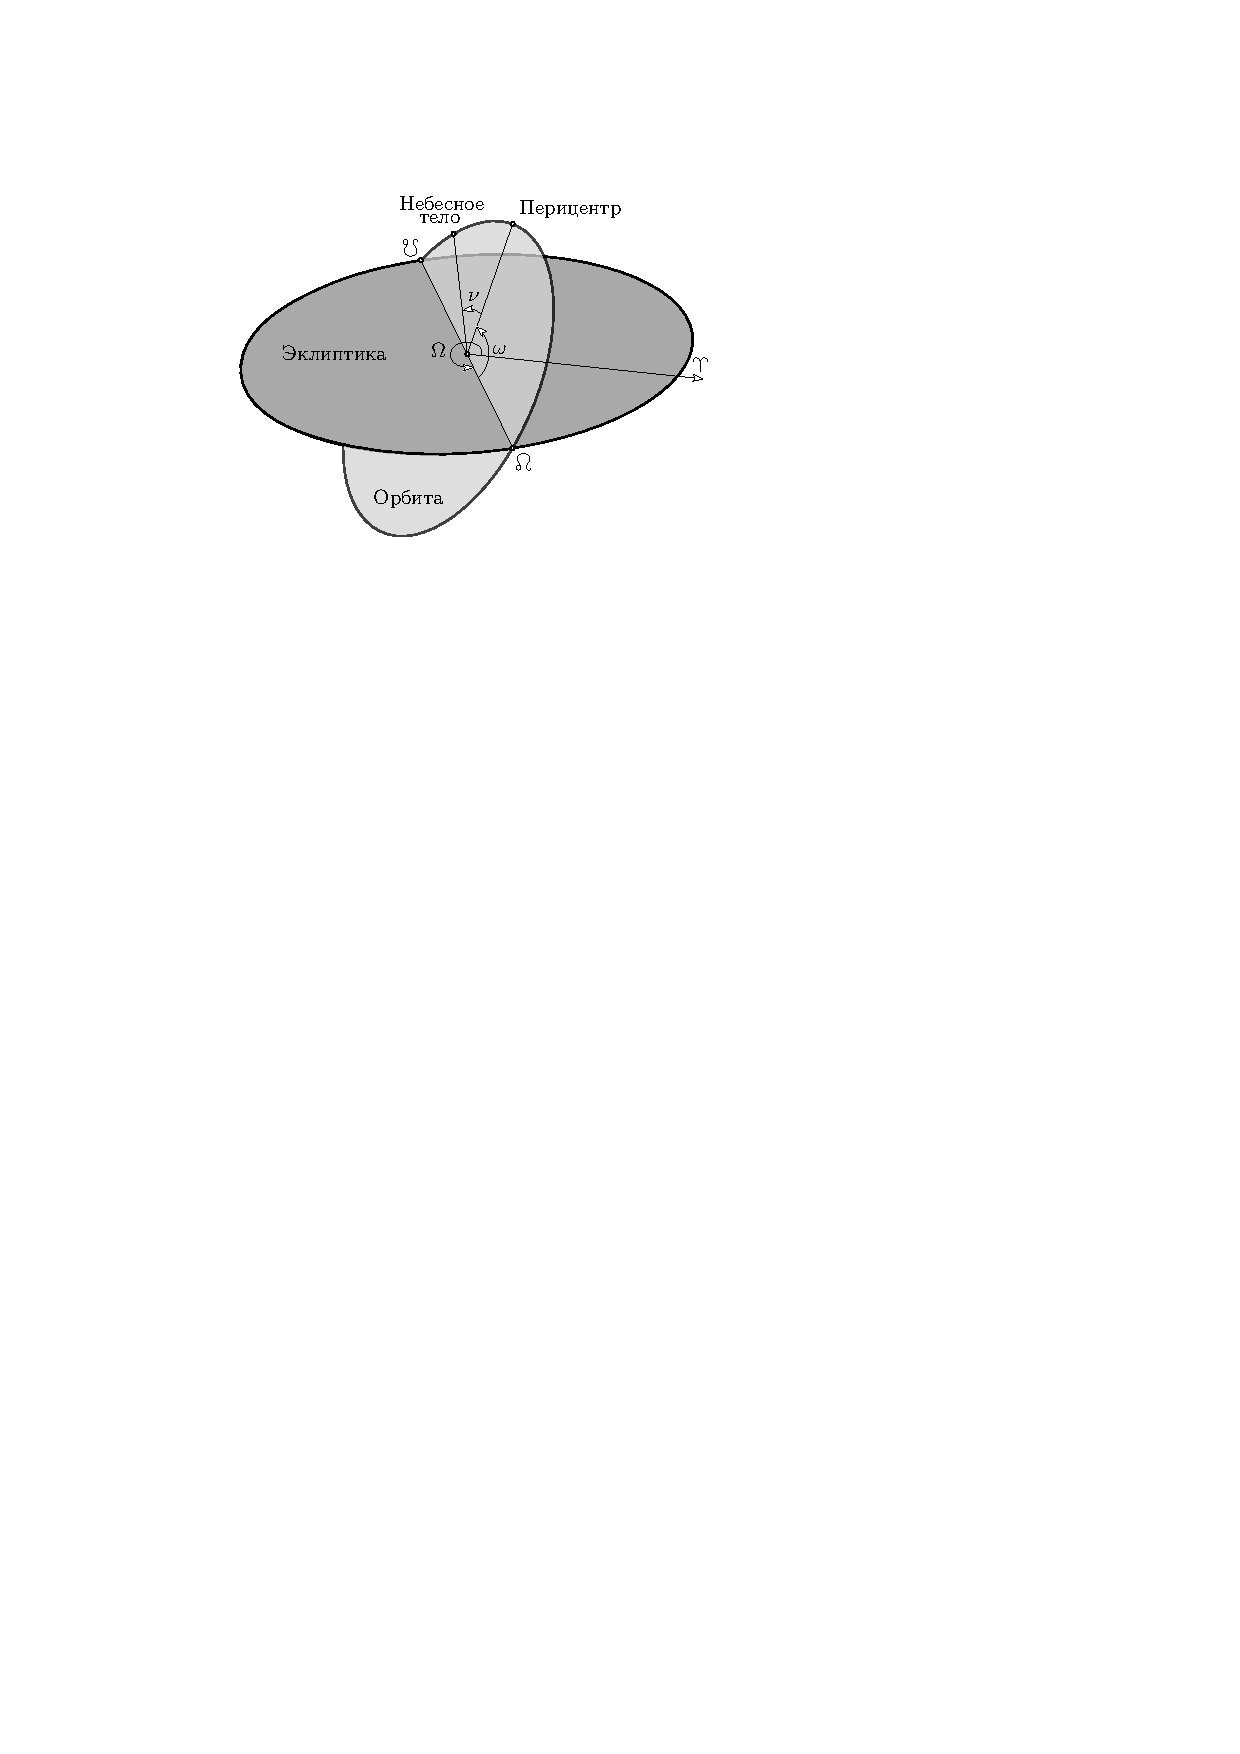
\includegraphics[width=.45\tw]{orbit-elem}
    \caption{Кеплеровы элементы орбиты}
    \label{fig:orb-elem}
\end{wrapfigure}
\term{Кеплеровы элементы} используют для описания положения в пространстве тел, находящихся на орбите вокруг заданного гравитирующего центра. Это шесть параметров: первые два из них определяют геометрию орбиты тела~--- это \imp{большая полуось} ($a$) и \imp{эксцентриситет} ($e$). Следующие три описывают положение орбиты в пространстве: \imp{наклонение} ($i$), \imp{аргумент перицентра} ($\omega$) и \imp{долгота восходящего узла} ($\Omega$). Последний~--- \imp{истинная аномалия} ($\nu$), задает положение тела на орбите.

Для использования кеплеровых элементов для описания положения тел первоначально необходимо задать систему отсчета~--- выбрать базовую плоскость, проходящую через гравитирующий центр и луч в этой плоскости, исходящий из него. Для описания положения тел Солнечной системы за базовую плоскость принимают плоскость эклиптики, а за луч~--- направление на точку весеннего равноденствия, при описании положения тел в околопланетном пространстве~--- плоскость экватора и луч, образованный пересечение экватора и нулевого меридиана.

\term{Истинная аномалия} тела, движущегося по орбите~--- угол в плоскости орбиты с вершиной в фокусе этой орбиты между направлениями на перицентр орбиты и на тело. Возрастает в ходе орбитального движения, изменяется в промежутке $[0^\circ, 360^\circ)$.

\term{Аргумент перицентра}~--- угол между направлениями на восходящий узел орбиты и на перицентр при наблюдении из притягивающего центра (фокуса орбиты). Откладывается в сторону орбитального движения, может иметь значению в промежутке $[0^\circ, 360^\circ)$.

\term{Наклонение}~--- это угол между плоскостью орбиты небесного тела и плоскостью эклиптики. Принимает значения от $0^\circ$ до $90^\circ$.

\term{Долгота восходящего узла}~--- угол в базовой плоскости между базовым направлением и направлением восходящий узел орбиты. Отсчитывается против часов стрелки при наблюдении из северного полупространства, лежит в промежутке $[0^\circ, 360^\circ)$.

\term{Узлы орбиты}~--- точки пересечения орбиты и базовой плоскости. \imp{Восходящий узел}~--- точка, в которой тело пересекает базовую плоскость при движении в северноим направлении, а \imp{нисходящий}~--- в южном.

Кеплеровы элементы являются \imp{углами Эйлера}, описывающими поворот абсолютно твердого тела в трёхмерном евклидовом пространстве. Введём прямоугольную декартову систему координат, связанную с орбитой тела: фокус~--- начало координат, направление на перицентр~--- ось~$x$, ось~$z$~--- нормаль к плоскости орбиты в северном полупространстве. Ось~$y$~--- луч в плоскости орбиты такой, чтобы направляющие вектора $\vec e_x$, $\vec e_y$ и $\vec e_z$ образовывали правую тройку. 

Найдём правила перехода из описанной системы координат в прямоугольную декартову систему координат, связанную с базовой плоскостью и лучом. Положение тела в орбитальной системе координат можно определить вектором $\vec r = (r \cos \nu, r \sin \nu, 0)$. Перейдем в систему координат, повернутую на угол $-\omega$ вокруг оси~$z$:
\begin{multline*}
    \vec r' = Z'_\omega\vec r 
    = \begin{pmatrix}
        \cos \omega & - \sin \omega & 0\\
        \sin \omega & \cos \omega & 0\\
        0 & 0 & 1
    \end{pmatrix} \begin{pmatrix}
        r \cos \nu\\
        r \sin \nu\\
        0
    \end{pmatrix} = \\
    = \begin{pmatrix}
        r \cos \nu \cos \omega - r \sin \nu \sin \omega\\
        r \cos \nu \sin \omega + r \sin \nu \cos \omega\\
        0
    \end{pmatrix} 
    =\begin{pmatrix}
        r \cos (\nu + \omega)\\
        r \sin (\nu + \omega)\\
        0
    \end{pmatrix}.
\end{multline*}
Ось~$x$ текущей системы координат совпадает с направлением на восходящий узел орбиты. Перейдем в систему координат, повернутую на угол $-i$ вокруг оси~$x$:
\begin{equation*}
    \vec r'' = X'_i\vec r' 
%    = X_{-i}Z_{-\omega}\vec r 
    = \begin{pmatrix}
        1 & 0 & 0\\
        0 & \cos i & - \sin i\\
        0 & \sin i & \cos i
    \end{pmatrix}\begin{pmatrix}
        r \cos (\nu + \omega)\\
        r \sin (\nu + \omega)\\
        0
    \end{pmatrix} 
    = \begin{pmatrix}
        r \cos (\nu + \omega)\\
        r \sin (\nu + \omega) \cos i\\
        r \sin (\nu + \omega) \sin i
    \end{pmatrix}.
\end{equation*}
Теперь ось~$z$ является нормалью к базовой плоскости. Повернём оси координат на угол $-\Omega$ вокруг оси $z$:
\begin{multline*}
    \vec r''' = Z'_\Omega\vec r''
%    = X_{-i}Z_{-\omega}\vec r 
    = \begin{pmatrix}
        \cos \Omega & - \sin \Omega & 0\\
        \sin \Omega & \cos \Omega & 0\\
        0 & 0 & 1
    \end{pmatrix}\begin{pmatrix}
        r \cos (\nu + \omega)\\
        r \sin (\nu + \omega) \cos i\\
        r \sin (\nu + \omega) \sin i
    \end{pmatrix} = \\
    = \begin{pmatrix}
        r \cos (\nu + \omega) \cos \Omega - r \sin (\nu + \omega) \cos i \sin \Omega\\
        r \cos (\nu + \omega) \sin \Omega + r \sin (\nu + \omega) \cos i \cos \Omega\\
        r \sin (\nu + \omega) \sin i
    \end{pmatrix}.
\end{multline*}

Отсюда следует, что координаты тела, находящегося на расстоянии~$r$ от фокуса, в базовой системе координат задаются соотношением
\begin{equation*}
    \vec r_0 =
%   r K \vec e_x \equiv
    r Z'_\Omega X'_i Z'_{\omega + \nu} \vec e_x =
    r \begin{pmatrix}
        \cos (\nu + \omega) \cos \Omega - \sin (\nu + \omega) \cos i \sin \Omega\\
        \cos (\nu + \omega) \sin \Omega + \sin (\nu + \omega) \cos i \cos \Omega\\
        \sin (\nu + \omega) \sin i
    \end{pmatrix}.
\end{equation*}








